\chapter{Experimental}
\section{Material}

\subsection{The Ag(100) crystal surface}
A \acf{Ag} single crystal from the Diamond Light Source with a crystal orientation of (100) was used as the substrate for the \ac{XPS} experiments. It is important that a single crystal is used, as this has a uniform and precisely defined surface and has almost no structural defects.

Silver forms a \ac{fcc} crystal system, which is shown in \autoref{fig:Ag(100)}. This corresponds to the Pearson symbol cF. In the crystal system of silver, one silver atom is surrounded by twelve others. Furthermore, Ag(100) does not reconstruct. The lattice constant of silver in the volume crystal is $4.0853\pm0.0013$~\si{\angstrom} at a temperature of $23\pm3$~\si{\celsius}\autocite{Liu1973}.

\begin{figure}[H]
	\centering
	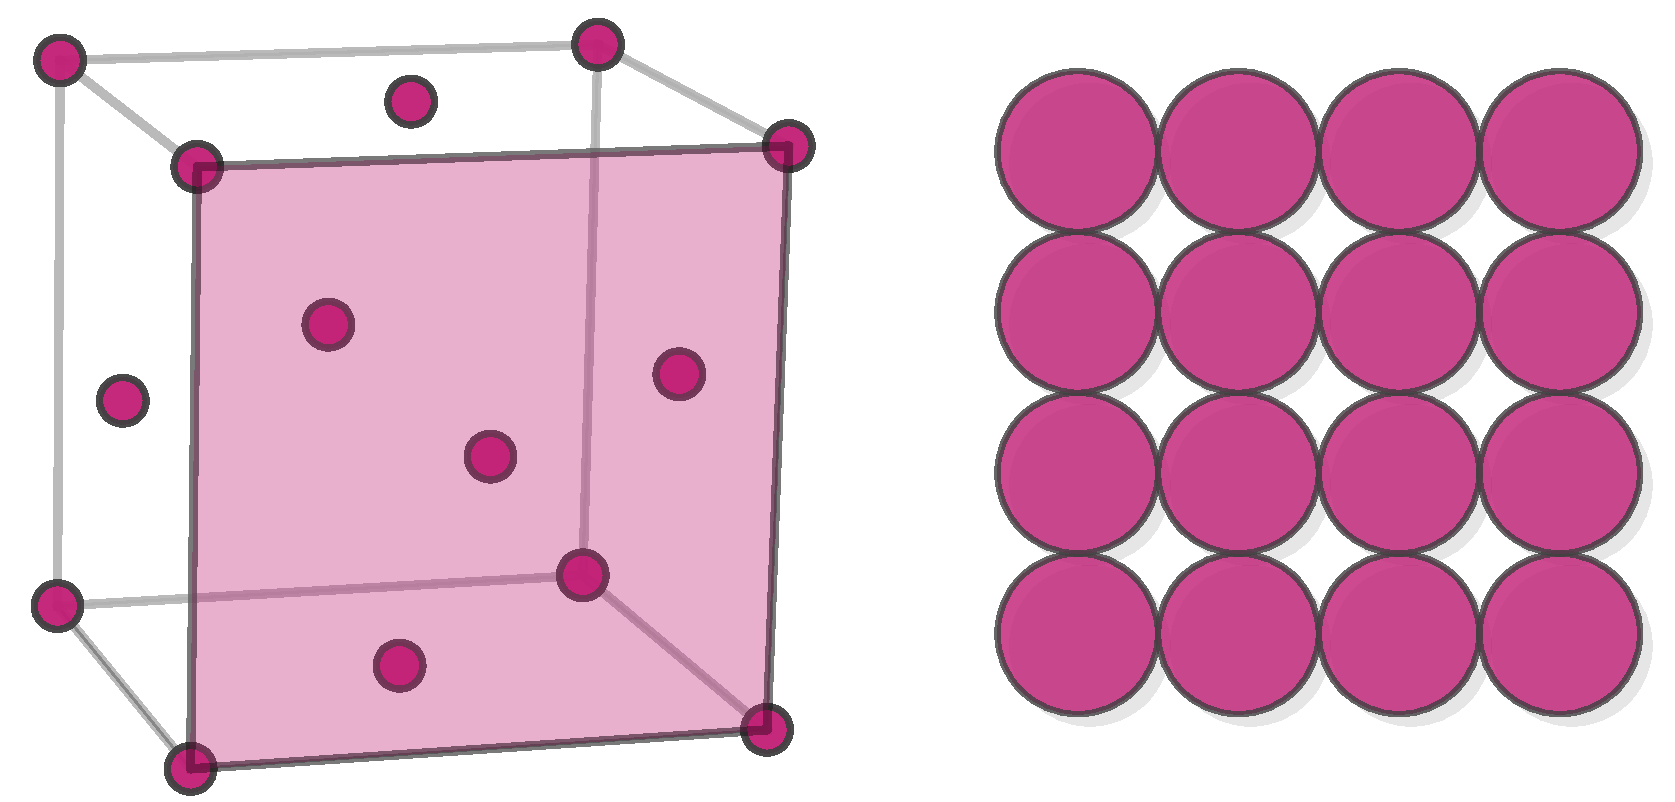
\includegraphics[width=0.9\textwidth]{images/Ag(100).pdf}
	\caption{Unit cell of the silver crystal with marked (100) plane and the Ag(100) surface with the unit cell vectors (black arrows) and the distinct adsorption sites (black circles).}
	\label{fig:Ag(100)}
\end{figure}

As seen in \autoref{fig:Ag(100)}, the unit cell of the Ag(100) surface is quadratic with a lattice constant $a_1=a_2=4.0853$~\si{\angstrom}/$\sqrt{2}=$2.8887~\si{\angstrom}. The Ag(100) surface has different adsorption sites called fcc, on-top and bridge. These sites are depicted as black circles in \autoref{fig:Ag(100)}.

\newpage
\section{Experimental setup}

All \ac{XPS} measurements were performed in an \ac{UHV} chamber at the I09 endstation at the Diamond Light Source in Didcot, UK, which is depicted in \autoref{fig:I09}.

\begin{figure}[htbp]
	\centering
	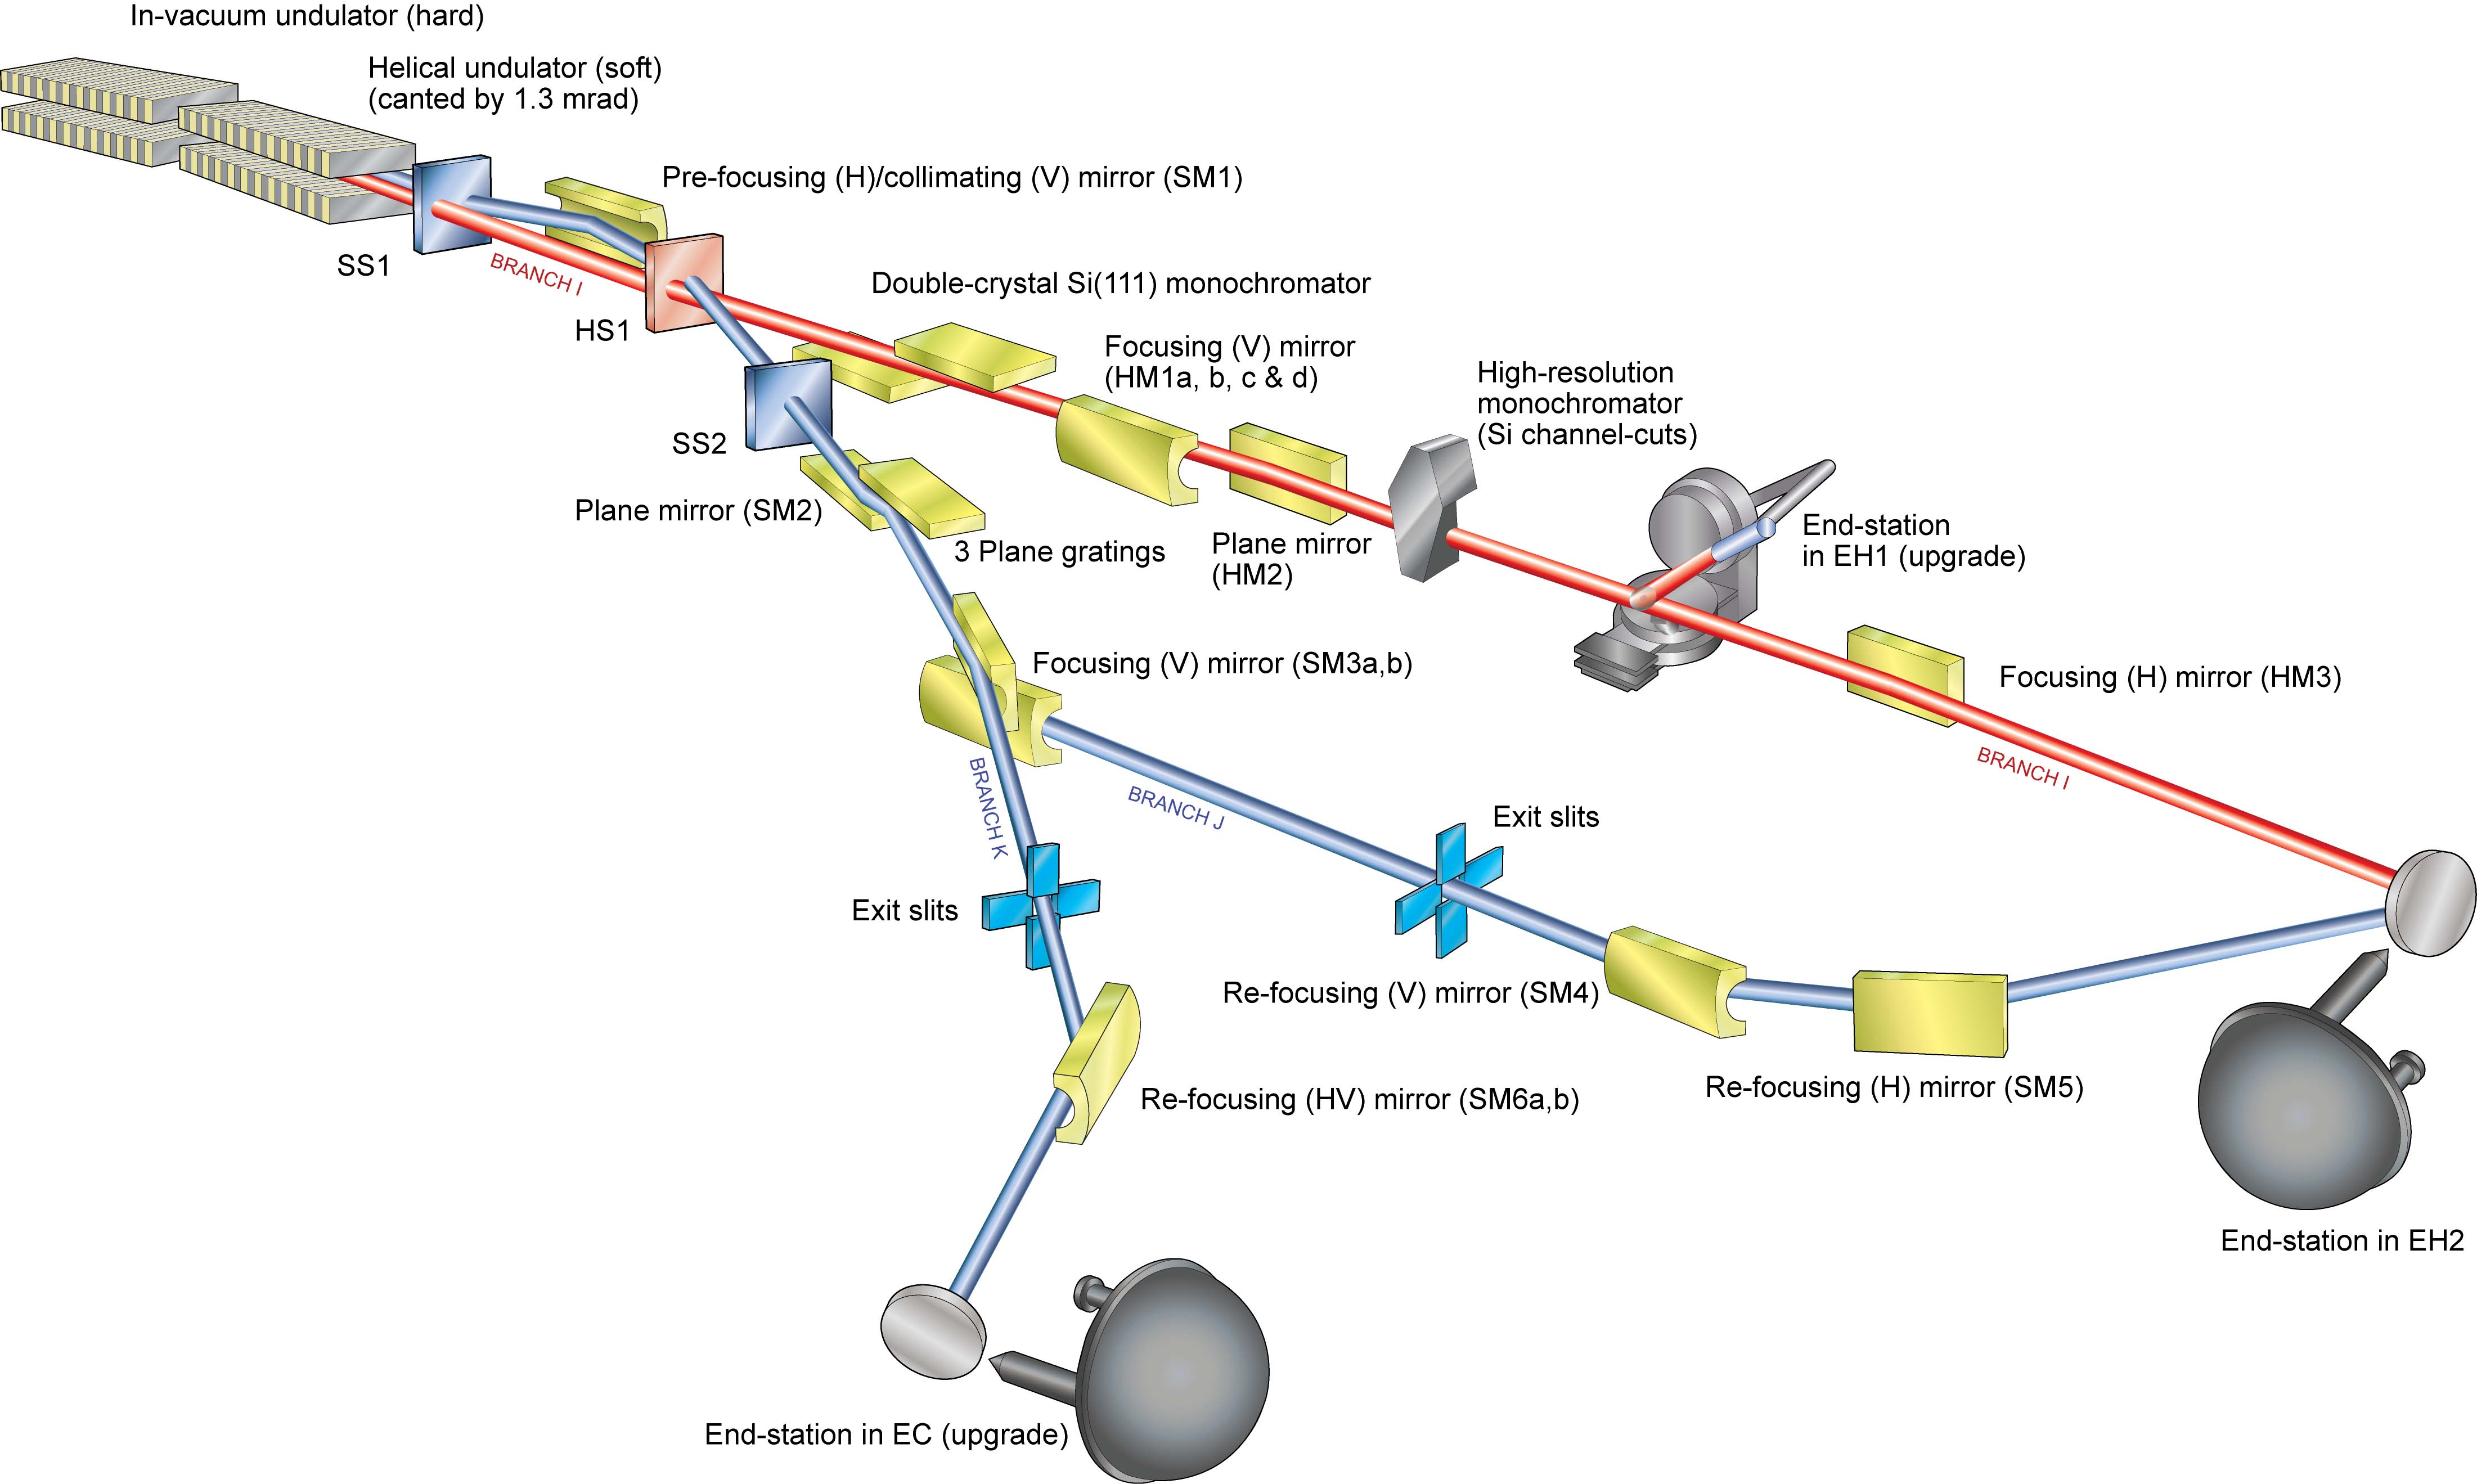
\includegraphics[width=0.9\textwidth]{images/I09.jpg}
	\caption{Schematic drawing of the I09 endstation of the Diamond Light Source in Didcot, UK. Picture taken from reference \cite{Diamond2025}.}
	\label{fig:I09}
\end{figure}

 This particular endstation utilizes radiation from an undulator located inside the electron storage ring of the synchrotron. The I09 endstation is equipped with a nitrogen-cooled Si(111) double crystal monochromator (hard x-rays) and a grating monochromator (soft x-rays). This setup enables high-intensity and precise x-ray measurements in the soft and hard x-ray ranges. The emitted photoelectrons were detected by a hemispherical EW4000 HAXPES analyzer purchased from Scienta Omicron. The analyzer has an acceptance cone of 56\si{\degree} and was mounted in the photon polarization plane.\autocite{Diamond2025} A schematic drawing of the sample position for the \ac{XPS} measurements is illustrated in \autoref{fig:experimental}.

\begin{figure}[htbp]
	\centering
	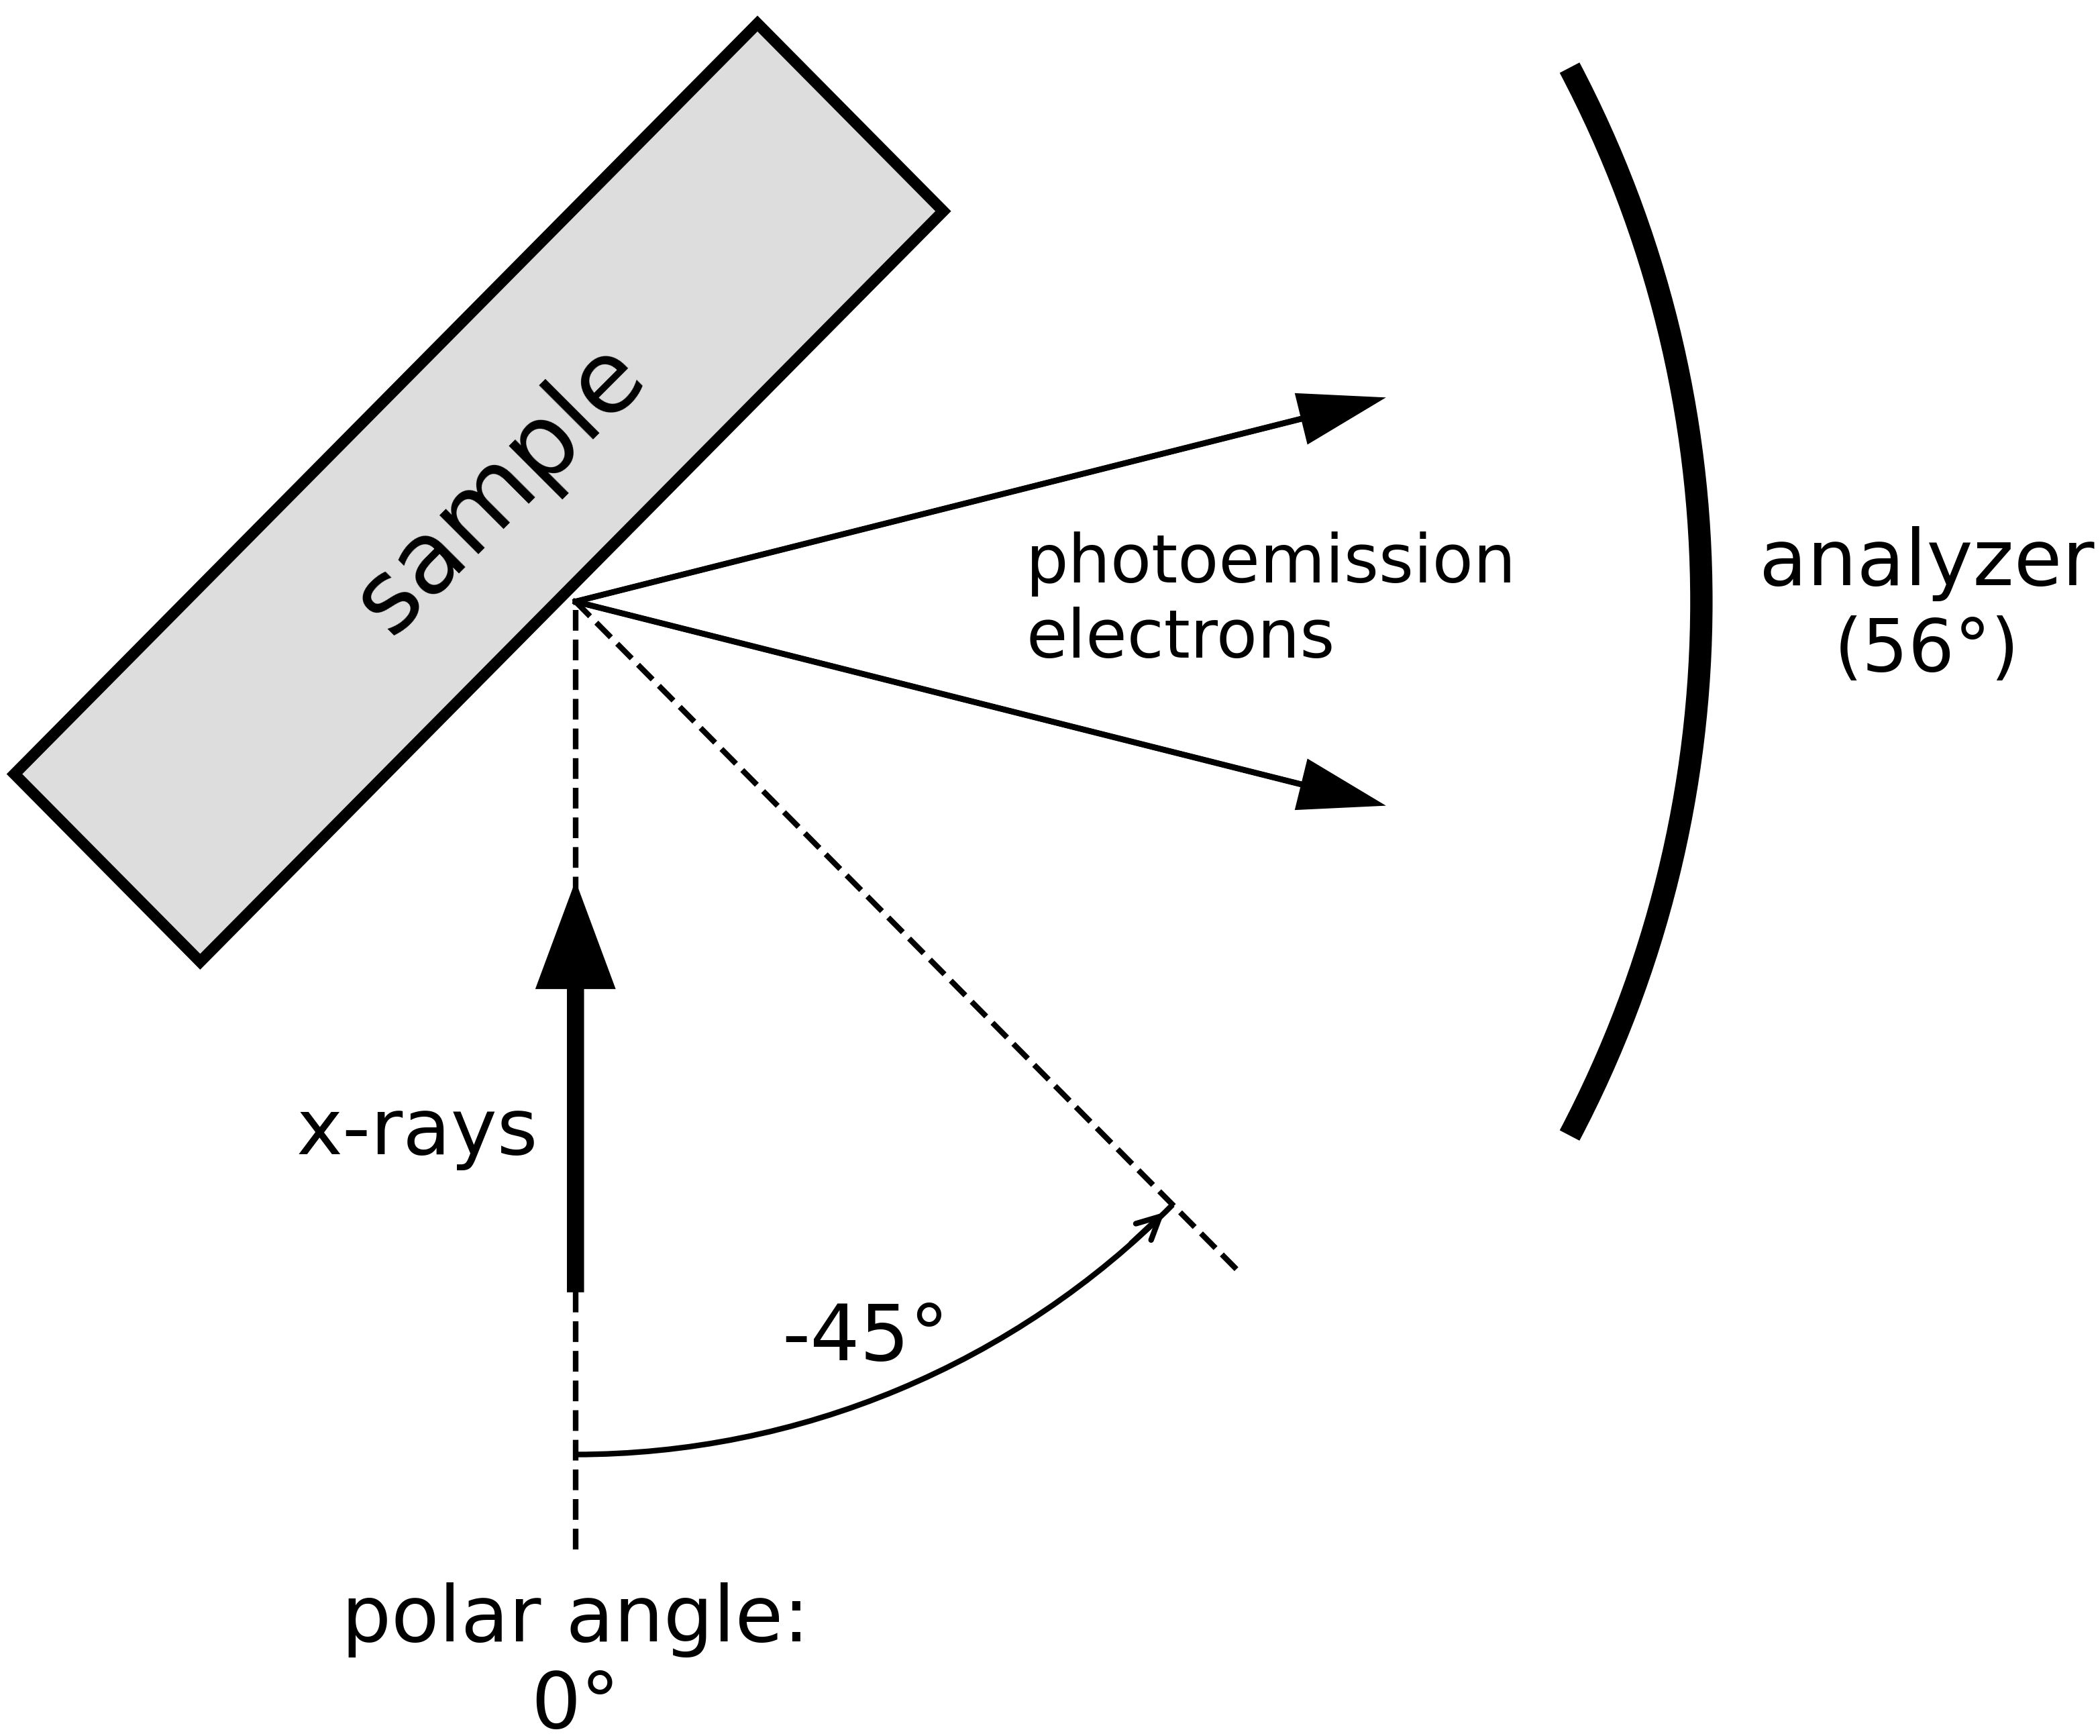
\includegraphics[width=0.6\textwidth]{images/experimental.png}
	\caption{Top view of the sample geometries for the \ac{XPS} measurements at the I09 endstation of the Diamond Light Source in Didcot, UK. Illustrated as in reference \cite{Kny2025}.}
	\label{fig:experimental}
\end{figure}

The experimental sample preparation is described in the following. First, the Ag(100) surface was cleaned by sputtering with argon ions. Therefore, argon was dosed into the chamber up to a pressure of $5\cdot 10^{-5}$~\si{mbar} and was accelerated with a voltage of 1~\si{keV}. Afterwards, the surface was heated up to 825~\si{K} for 45~\si{min} to increase the thermal diffusion and heal defects on the Ag(100) surface.

Subsequently, \ac{QA} was evaporated onto the Ag(100) surface with the sample being at room temperature. Therefore, the evaporator was heated to about 500~\si{\degreeCelsius}. The deposition process was performed according to procedures derived in the lab in Bonn, where the depostion could be controlled by a mass spectrometer and \ac{SPA-LEED} measurements. After evaporation, the phase of the \ac{QA} molecules was characterized using \ac{LEED}.

For the measurements of the \ac{XPS} spectra, soft x-ray radiation with an energy of either 500~\si{\eV} for C1s and N1s or 630~\si{\eV} for O1s was used. Therefore, the sample was rotated by -45\si{\degree} in the polar direction towards the analyzer.

The detailed parameters for the data acquistion are listed in \autoref{tab:experimental}. The pass energy $E_\mathrm{pass}$ of the analyzer determines the kinetic energy of the photoelectrons and therefore the energy resolution of the measurement. The step width is the energy difference between two consecutive data points in the \ac{XPS} spectrum. The number of frames is the number of times the same spectrum was measured and averaged to reduce noise in the data.

\begin{table}[H]
	\centering
	\caption{Experimental parameters for \ac{XPS} measurements at the I09 endstation of the Diamond Light Source in Didcot, UK.}
	\begin{tabular}{|c|c|c|c|c|}
		\hline
		& photon energy $E_\mathrm{\gamma}$ & pass energy $E_\mathrm{pass}$ & step width & number of frames \\
		\hline
		C1s & 500~\si{\eV} & 20~\si{\eV} & 40~\si{meV} & 17 \\
		\hline
		O1s & 630~\si{\eV} & 20~\si{\eV} & 40~\si{meV} & 17 \\
		\hline
		N1s & 500~\si{\eV} & 20~\si{\eV} & 40~\si{meV} & 17 \\
		\hline
	\end{tabular}
	\label{tab:experimental}
\end{table}

The parameters for the measurements were chosen to achieve a good signal-to-noise ratio and a high energy resolution. Furhtermore, the acquisiton time for each spectrum was as short as possible to prevent beam damage of the sample. 

\ac{XPS} spectra for the Fermi energy $E_\mathrm{F}$ was measured after each \ac{XPS} measurement of C1s, O1s and N1s to ensure that the \ac{BE} of the measured spectra is referenced against the Fermi level. $E_\mathrm{F}$ was measured with the same photon energy as the corresponding component and a pass energy of 20~\si{\eV}. The step width was set to 40~\si{meV} and the number of frames was changed for each measurement.

\section{Data processing}

The measured data were then subjected to an initial processing stage, whereby the values from multiple datasets employing identical settings for the measurements were averaged to obtain an increased signal-to-noise ratio. Subsequently, the data underwent further processing with the software CasaXPS.\autocite{CasaSoftwareLtd2022} Each XPS spectrum was processed in a consistent manner, as outlined below.

Initially, the \ac{BE} of the \ac{XPS} spectrum was calibrated against the Fermi energy $E_\mathrm{F}$. Small inaccuracies of all measurement devices may lead to inaccuracies in the \ac{BE}. Therefore, an \ac{XPS} spectrum of the Fermi edge with same photon energy as the corresponding component \ac{XPS} spectrum is used and fitted with a Fermi function. Without inaccuracies of the devices, $E_\mathrm{F}$ should be zero and for this reason the obtained Fermi energy is then used for the \ac{XPS} spectrum of the component to calibrate the \ac{BE}.

Therefore, the binding energy was shifted by the value of the Fermi energy, which was determined from the Fermi edge. This ensures that the \ac{BE} of the measured \ac{XPS} spectra is referenced against the Fermi level $E_\mathrm{F}$.

Afterwards, a linear background was fitted to the raw and averaged data. This background is then substracted for further data processing. Afterwards, the corresponding fitting models from \autoref{sec:results} were applied. Therefore, the different peaks with line shape and constraints from \autoref{tab:casa} were used. These settings are the same for each processed dataset.
Subsequently, the processed data was then exported from CasaXPS and illustrated using a customized python script, enabling the generation of various plots as outlined in \autoref{sec:results}.


\begin{table}[H]
	\centering
	\caption{Used parameter in CasaXPS\autocite{CasaSoftwareLtd2022} for the different peaks of the \ac{XPS} spectra of \ac{QA} on Ag(100) at the I09 endstation of the Diamond Light Source in Didcot, UK.}
\begin{tabular}{|c|c|c|}
	\hline
	~~~~~~peak~~~~~~ & ~~~~~~line shape~~~~~~ & ~~~~~~area constraint~~~~~~ \\
	\hline
	$\mathrm{C_{arom}}$ & LA(1,8,800) & 10 \\
	\hline
	$\mathrm{C_{NH}}$ & LA(1,8,800) & 4 \\
	\hline
	$\mathrm{C_{CO}}$ & LA(1,8,800) & 4 \\
	\hline
	$\mathrm{C_{O}}$ & LA(1,8,200) & 2 \\
	\hline \hline
	O1 & LA(1,8,400) & 1 (for $\beta$-phase) \\
	\hline
	$\mathrm{O1_{sat}}$ & LA(1,1,400) &  \\
	\hline
	O2 & LA(1,8,400) & 1 (for $\beta$-phase) \\
	\hline
	$\mathrm{O2_{sat}}$  & LA(1,1,400) &  \\
	\hline \hline
	N1 & LA(1,8,400) & 1 (for $\beta$-phase) \\
	\hline
	$\mathrm{N1_{damage}}$  & LA(1,8,400) &  \\
	\hline
	N2 & LA(1,8,400) & 1 (for $\beta$-phase) \\
	\hline
\end{tabular}
	\label{tab:casa}
\end{table}

Explain different line shapes and area constraints

\cleardoublepage
